\documentclass[11pt]{article}
\usepackage[margin=1in]{geometry}
\usepackage[T1]{fontenc}
\usepackage{mathptmx}
\usepackage{courier}
\usepackage{amsmath}
\usepackage{graphicx}
\usepackage{booktabs}
\usepackage{caption}
\usepackage[shortlabels]{enumitem}
\usepackage[hidelinks]{hyperref}
\captionsetup{font=small,labelfont=bf}

\title{Filtered, Not Faked: Beauty Filters and Skin-Tone Disparities\\in Deepfake Detection}
\author{Tanishk Gangwar, Garv, Shhorya Agarwal\\[4pt]
\small Department of Data Science and Engineering, Manipal University Jaipur\\
\small DSE3140 Computer Vision\\
\small Contact: \texttt{tanishk7531@gmail.com}}
\date{October 2026}

\begin{document}
\maketitle

\begin{abstract}
Beauty filters that smooth and lighten skin are applied by default in many phone cameras, yet deepfake detectors, and fairness audits of those detectors, are evaluated on unfiltered images. We test whether filtering causes real faces to be flagged as deepfakes, and whether the effect falls harder on darker skin. We apply skin smoothing, skin lightening and their combination at controlled strengths to 2,100 real FairFace faces (300 per race group, seven groups), measure skin tone with the Individual Typology Angle (ITA), and score every version with a pretrained deepfake detector at a fixed threshold. Because filter strength is set by the experimenter, the dose-response estimates are causal. Full-strength smoothing raises the false-positive rate from 5.0\% to 17.0\%. The absolute increase is 10.9 percentage points larger for the darkest third of faces than for the lightest third (95\% CI 6.9 to 14.5), although on the odds scale the interaction is not significant ($p=0.10$). Unfiltered Indian faces are flagged most of any group (9.7\%), rising to 29.7\% under smoothing. Lightening alone does not raise false positives. Finally, we show a measurement problem: lightening moves 87\% of faces into a different skin-tone band, so an audit that reads skin tone off the filtered image reports a false-positive rate of 4.8\% for the darkest band when the true rate for those people is 11.1\%.
\end{abstract}

\section{Introduction}
Deepfake detectors are increasingly used in content moderation and identity verification, where a false positive means a real person's photo is called fake. Prior work shows these detectors have unequal error rates across demographic groups \cite{trinh2021,hazirbas2021,xu2022}, and separately that beauty filters degrade detection \cite{libourel2024,concas2025}. No study has connected the two. Beauty filtering, especially skin lightening, is common in South Asian phone cameras and apps, and it changes exactly the attribute that fairness audits measure.

We ask three research questions:
\begin{enumerate}[label=\textbf{RQ\arabic*.}, leftmargin=*]
  \item Does applying a beauty filter to a real face increase the probability that a detector flags it as a deepfake?
  \item Is that increase larger for darker skin tones?
  \item How much does skin lightening move faces between skin-tone groups, and how much does that distort per-group fairness metrics?
\end{enumerate}

Our contributions are (i) a controlled dose-response design that makes RQ1 and RQ2 causal claims, (ii) evidence on 2,100 real faces that smoothing causes false positives and that the absolute harm is largest for darker skin and for Indian faces, (iii) a quantification of the measurement problem in RQ3, and (iv) an open-source evaluation pipeline.

\section{Related Work}
\textbf{Demographic bias in deepfake detectors.} Trinh and Liu found error-rate gaps of up to 10.7\% across racial groups \cite{trinh2021}. Hazirbas et al.\ found DFDC-winning models performed worse on darker-skinned subjects \cite{hazirbas2021}. Xu et al.\ annotated five datasets with 47 attributes and found strong bias \cite{xu2022}, and Nadimpalli and Rattani found gender gaps \cite{gbdf2022}. In contrast, Panda et al.\ found no systematic bias for pretrained checkpoints on diffusion-generated images \cite{panda2026}. All of these audit unprocessed benchmark images.

\textbf{Fairness-aware detectors.} Lin et al.\ showed fair loss functions do not stay fair across domains and proposed disentangled features with a flattened loss landscape \cite{lin2024}. Cheng et al.\ used back-door adjustment to link fairness and generalization \cite{cheng2025}. Both treat demographic labels as fixed properties of an image.

\textbf{Beauty filters and detection.} Libourel et al.\ built Celeb-DF-B by applying social-media filters and found a notable AUC drop \cite{libourel2024}. Concas et al.\ found filtering real images can make detectors call them fake \cite{concas2025}. Both report aggregate performance on Western celebrity data, with no skin-tone analysis and no lightening filter.

\textbf{Gap.} No prior work tests skin-modifying filters per skin tone under controlled strengths, and, to our knowledge from a targeted search, none observes that such filters alter the group label used to compute fairness metrics.

\section{Method}
Every image in the study is a real photograph, so every ``fake'' prediction is a false positive.

\textbf{Data.} We use 300 real faces per race group from the FairFace validation split \cite{fairface} (7 groups, 2,100 faces, including the Indian group), resized to $224\times224$.

\textbf{Skin tone.} We compute the Individual Typology Angle \cite{chardon1991} on skin pixels in the central face region, taking the median over pixels:
\begin{equation}
\mathrm{ITA} = \arctan\left(\frac{L^* - 50}{b^*}\right)\times\frac{180}{\pi}
\end{equation}
where $L^*$ and $b^*$ are CIELAB coordinates. Faces are assigned to six standard bands: very light ($>55^\circ$), light (41 to $55^\circ$), intermediate (28 to $41^\circ$), tan (10 to $28^\circ$), brown ($-30$ to $10^\circ$) and dark ($<-30^\circ$). Faces with fewer than 50 detected skin pixels get no ITA value.

\textbf{Treatments.} We apply three filters at strengths $s\in\{0, 0.5, 1.0\}$, where $s=0$ is the control. Each acts only on skin, selected by a soft mask from the YCrCb thresholds $133\le Cr\le173$, $77\le Cb\le127$:
\begin{itemize}[leftmargin=*]
  \item \textbf{Smooth:} an edge-preserving bilateral filter whose kernel size and sigma grow with $s$, blended in proportion to $s$.
  \item \textbf{Lighten:} raise $L^*$ by $25s$ and scale $a^*$ by $(1-0.25s)$ to reduce redness, as commercial whitening effects do.
  \item \textbf{Smooth + lighten:} smoothing followed by lightening at the same strength.
\end{itemize}
Every version, including the control, is saved as JPEG at quality 85, so compression is held constant across arms \cite{grommelt2024}. Figure~\ref{fig:example} shows one face under all nine settings.

\begin{figure}[t]
\centering
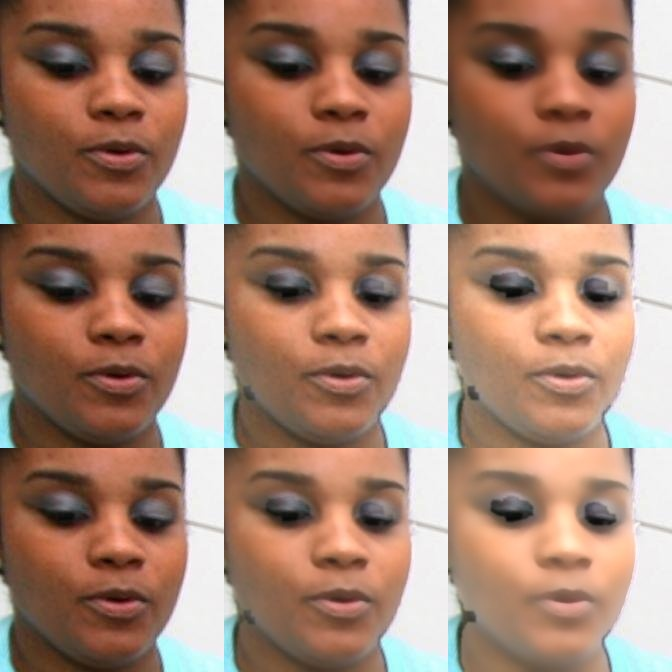
\includegraphics[width=0.45\linewidth]{fig_example.jpg}
\caption{One FairFace face under each treatment. Rows: smooth, lighten, smooth + lighten. Columns: strength 0 (control), 0.5, 1.0.}
\label{fig:example}
\end{figure}

\textbf{Detection.} We score each version with a pretrained ViT deepfake detector, Deep-Fake-Detector-v2 \cite{detector}, whose classes are Realism and Deepfake. The decision threshold is set once on unfiltered images for a pooled false-positive rate (FPR) of 5\% (threshold 0.745), then held fixed, as a deployed system would. The full run produced 18,900 scores and took 7 minutes on one T4 GPU.

\textbf{Pre-specified analysis.} We report FPR per ITA band and per FairFace race group at each strength, with 95\% bootstrap confidence intervals (1,000 resamples). For RQ2, we fit a logistic model per filter with standard errors clustered by image:
\begin{equation}
\mathrm{logit}\,P(\text{flagged}) = \beta_0 + \beta_1 s + \beta_2\,\mathrm{ITA}_z + \beta_3\,(s\times\mathrm{ITA}_z)
\label{eq:logit}
\end{equation}
where $\mathrm{ITA}_z$ is standardized skin tone. A negative $\beta_3$ means the filter raises false positives more for darker skin, on the odds scale. Because $s$ is assigned by us rather than observed, $\beta_3$ has a causal reading. For RQ3, we re-measure ITA on each filtered image and report the share of faces whose band changes, and compare FPR grouped by true (pre-filter) band against FPR grouped by the band an auditor would read off the filtered image.

\textbf{Secondary analysis (added after the main run).} On these in-the-wild photos, absolute ITA values run dark: the median ITA of White faces is about $0^\circ$, which the standard bands call brown (Section~\ref{sec:limits}). We therefore also group faces into thirds of the sample's own ITA distribution (cut points $-39.8^\circ$ and $1.3^\circ$; 677 faces per third), which depends only on the ordering of skin tones. Because the logistic interaction in Equation~\ref{eq:logit} measures relative change, we also report the absolute change in FPR from $s=0$ to $s=1$ per third, with a 2,000-resample bootstrap CI for the darkest-minus-lightest gap, and a linear probability version of Equation~\ref{eq:logit} with the same clustered errors. These analyses were not planned before the run and are reported as such.

\section{Pipeline Verification on Synthetic Data}
Before running on real faces, we verified each component on 180 synthetic test images (textured skin-coloured ellipses in six tones) with a training-free stand-in detector that scores an image as more ``fake'' the less high-frequency texture it has. These numbers are not findings about deepfake detection. They confirmed that ITA bands follow the input tones in order, that the stand-in's flag rate rises with smoothing but not with lightening, and that lightening moves faces between bands (87.2\% at full strength) while smoothing does not (2.2\%).

\section{Results}

\subsection{RQ1: Smoothing causes false positives}
Table~\ref{tab:pooled} gives the pooled FPR over all 2,100 faces. Smoothing raises it from 5.0\% to 8.0\% at half strength and 17.0\% at full strength, an odds ratio of 4.1 per unit of strength ($p<10^{-40}$). The combined filter raises it to 9.2\%. Lightening alone does not raise it: FPR falls slightly, to 3.9\%. The answer to RQ1 is yes for smoothing and no for lightening alone.

\begin{table}[h]
\centering
\caption{Pooled false-positive rate (\%) by filter and strength, and the strength effect from Equation~\ref{eq:logit} (odds ratio per unit of strength, at mean skin tone). $n=2{,}100$ faces.}
\label{tab:pooled}
\begin{tabular}{lrrrrr}
\toprule
Filter & $s=0$ & $s=0.5$ & $s=1.0$ & OR & $p$ \\
\midrule
Smooth           & 5.0 & 8.0 & 17.0 & 4.11 & $3\times10^{-42}$ \\
Lighten          & 5.0 & 4.2 & 3.9  & 0.78 & 0.029 \\
Smooth + lighten & 5.0 & 7.1 & 9.2  & 1.98 & $3\times10^{-9}$ \\
\bottomrule
\end{tabular}
\end{table}

\subsection{RQ2: Darker skin bears the largest absolute increase}
Even unfiltered, the detector flags darker faces more often: the darkest third has an FPR of 6.4\% against 3.8\% for the lightest (odds ratio 0.76 per SD of higher ITA, $p=0.011$). Figure~\ref{fig:tertile} and Table~\ref{tab:tertile} show how each filter changes this.

\begin{figure}[t]
\centering
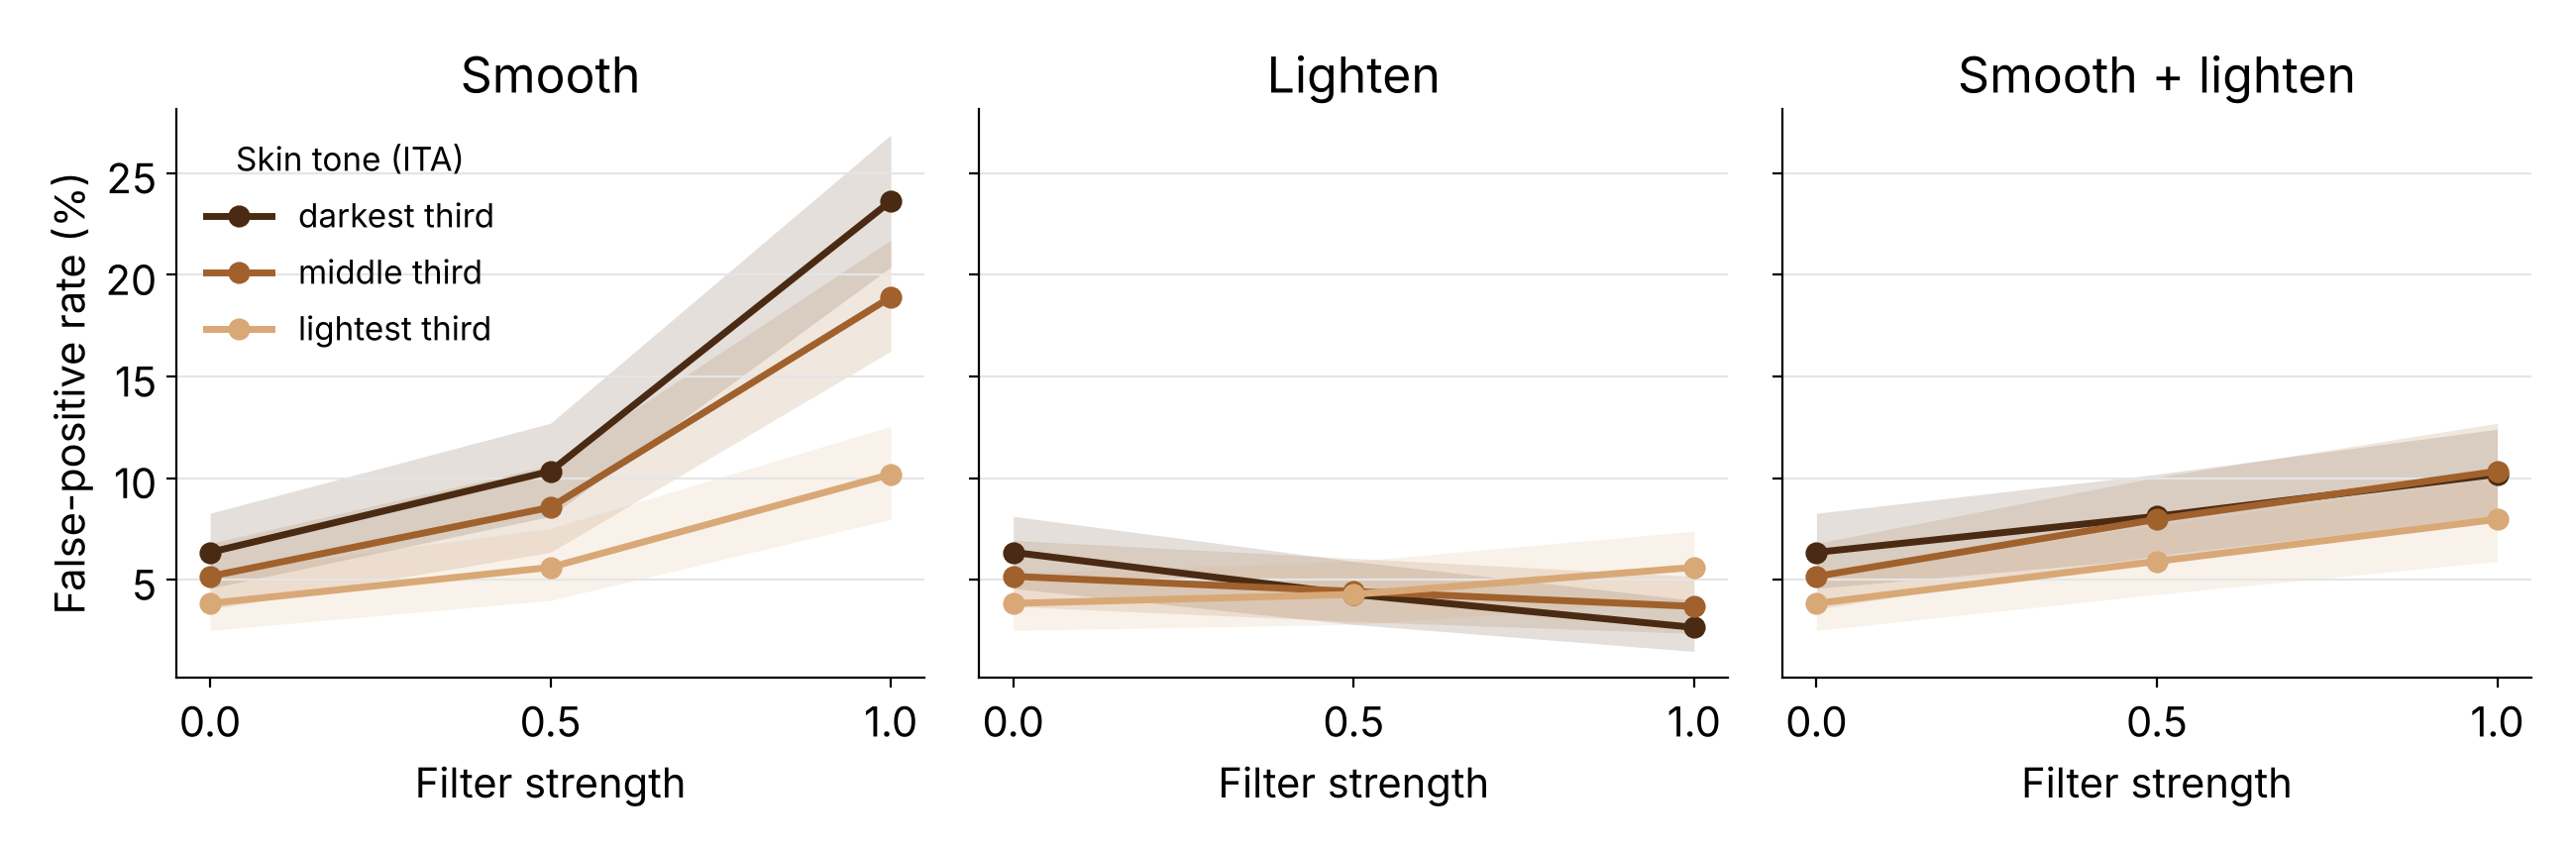
\includegraphics[width=\linewidth]{fig_tertile_dose.png}
\caption{False-positive rate against filter strength, by thirds of measured skin tone (ITA). Shaded bands are 95\% bootstrap CIs. 677 faces per third.}
\label{fig:tertile}
\end{figure}

\begin{table}[h]
\centering
\caption{FPR (\%) by skin-tone third at $s=0$ and $s=1.0$ with 95\% CIs, the change in percentage points, and the darkest-minus-lightest gap in that change.}
\label{tab:tertile}
\small
\begin{tabular}{llrrr}
\toprule
Filter & Third & $s=0$ & $s=1.0$ & Change \\
\midrule
Smooth & Darkest  & 6.4 [4.6, 8.3] & 23.6 [20.4, 26.9] & +17.3 \\
       & Middle   & 5.2 [3.5, 6.8] & 18.9 [16.2, 21.7] & +13.7 \\
       & Lightest & 3.8 [2.5, 5.3] & 10.2 [8.0, 12.6]  & +6.4 \\
       & \multicolumn{3}{l}{Gap, darkest minus lightest [95\% CI]} & \textbf{+10.9 [6.9, 14.5]} \\
\midrule
Lighten & Darkest  & 6.4 [4.6, 8.1] & 2.7 [1.5, 4.0] & $-3.7$ \\
        & Middle   & 5.2 [3.7, 6.9] & 3.7 [2.4, 5.2] & $-1.5$ \\
        & Lightest & 3.8 [2.5, 5.3] & 5.6 [4.0, 7.4] & +1.8 \\
        & \multicolumn{3}{l}{Gap, darkest minus lightest [95\% CI]} & $-5.5$ [$-7.8$, $-3.4$] \\
\midrule
Smooth + lighten & Darkest  & 6.4 [4.6, 8.3] & 10.2 [8.1, 12.4] & +3.8 \\
                 & Middle   & 5.2 [3.5, 6.8] & 10.3 [8.1, 12.7] & +5.1 \\
                 & Lightest & 3.8 [2.5, 5.3] & 8.0 [5.9, 10.0]  & +4.1 \\
                 & \multicolumn{3}{l}{Gap, darkest minus lightest [95\% CI]} & $-0.3$ [$-3.7$, 3.0] \\
\bottomrule
\end{tabular}
\end{table}

\textbf{Smoothing.} The darkest third rises by 17.3 points and the lightest by 6.4, a gap of 10.9 points (95\% CI 6.9 to 14.5). The linear probability model agrees ($p=3\times10^{-10}$). On the odds scale, however, the pre-specified interaction is not significant (OR 0.84 per SD of ITA, $p=0.10$). The two scales answer different questions. Smoothing multiplies the odds of being flagged by a similar factor for everyone, but darker faces start from a higher baseline, so they lose about 2.7 times as much in absolute terms. For the person whose photo is rejected, the absolute rate is the one that matters.

\textbf{Lightening} reverses the pattern: it lowers FPR for the darkest third (6.4\% to 2.7\%) and slightly raises it for the lightest (3.8\% to 5.6\%). The odds-scale interaction is significant (OR 1.74, $p=1.5\times10^{-6}$). Making darker skin lighter makes this detector less likely to call it fake, which is consistent with its baseline tendency to flag darker faces. Under the combined filter the two effects roughly cancel and the thirds do not differ (gap $-0.3$, CI $-3.7$ to 3.0; odds-scale $p=0.25$).

\textbf{By race group.} Table~\ref{tab:groups} reports FPR by FairFace label. Indian faces are flagged most both unfiltered (9.7\%) and under full smoothing (29.7\%, CI 24.7 to 35.0), against 8.7\% for White faces. Black faces, which have the lowest median ITA ($-52^\circ$), start among the lowest (3.0\%). Group differences are therefore not explained by measured skin tone alone; the detector responds to something else that varies across these groups, which this study cannot identify.

\begin{table}[h]
\centering
\caption{FPR (\%) by FairFace race label, unfiltered and under full smoothing, with 95\% bootstrap CIs. 300 faces per group.}
\label{tab:groups}
\begin{tabular}{lrr}
\toprule
Group & Unfiltered & Smooth, $s=1.0$ \\
\midrule
Indian          & 9.7 [6.3, 13.0] & 29.7 [24.7, 35.0] \\
Middle Eastern  & 7.3 [4.3, 10.3] & 18.3 [14.0, 22.7] \\
Latino/Hispanic & 3.3 [1.7, 5.3]  & 17.3 [13.0, 21.3] \\
Black           & 3.0 [1.3, 5.0]  & 16.3 [12.3, 20.3] \\
Southeast Asian & 3.3 [1.3, 5.7]  & 16.0 [12.3, 20.7] \\
East Asian      & 4.3 [2.3, 7.0]  & 13.0 [9.3, 16.7] \\
White           & 4.0 [2.0, 6.3]  & 8.7 [5.7, 12.0] \\
\bottomrule
\end{tabular}
\end{table}

\subsection{RQ3: Lightening distorts the audit}
Lightening moves 66.1\% of faces into a different ITA band at half strength and 87.4\% at full strength (smooth + lighten: 65.3\% and 87.3\%). Smoothing alone moves 1.3\% and 3.0\%, close to the 0.5\% that JPEG re-encoding moves at $s=0$ (Figure~\ref{fig:shift}).

This shift distorts per-group error rates. Under full smooth + lighten, an auditor who reads skin tone off the filtered image reports an FPR of 4.8\% for the dark band, while the true FPR for faces that are dark before filtering is 11.1\%: more than half of the harm to that group disappears from the audit. The errors do not vanish; they are reassigned to lighter bands, whose apparent FPR rises (brown 8.6\% true vs 13.8\% seen; light 5.0\% vs 8.1\%). Under smoothing alone, which barely moves faces, the true and seen rates differ by at most 1.5 points.

\begin{figure}[t]
\centering
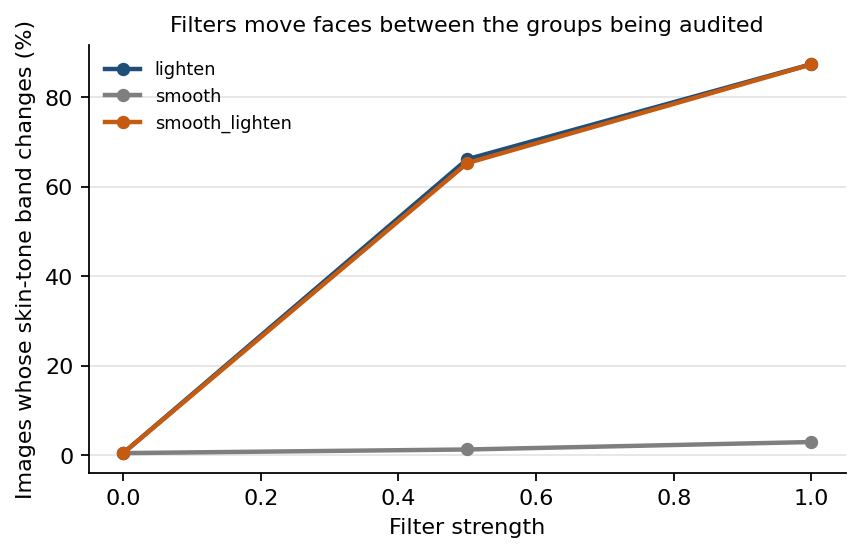
\includegraphics[width=0.6\linewidth]{fig_label_shift.png}
\caption{Share of faces whose ITA band changes after filtering.}
\label{fig:shift}
\end{figure}

\section{Discussion and Limitations}
\label{sec:limits}
\textbf{Implications.} Deployers should test detectors on filtered images, since default beauty modes alone can triple false positives. Fairness audits should label demographic attributes from unmodified source images or from the person, never from the image being scored, or skin-lightening filters will hide the very disparity the audit is meant to find. Reporting both absolute and relative disparities avoids the ambiguity seen in RQ2, where the two scales give different answers.

\textbf{Limitations.} (1) We use one public community detector rather than a standard benchmark checkpoint such as Xception; results may not transfer. (2) ITA is computed automatically and is sensitive to lighting and white balance. On FairFace, absolute values run dark (median ITA $-21.1^\circ$ overall, about $0^\circ$ for White faces), so the textbook band names should not be read literally; we rely on relative thirds for skin-tone comparisons. The ordering is plausible (Black faces lowest, White highest), but human Monk Skin Tone labels would be stronger. (3) 3.3\% of faces had too few detected skin pixels for an ITA value (1.7\% to 5.0\% by group) and are excluded from skin-tone analyses. (4) Our filters approximate commercial beauty modes but are not identical to them; validating on photos taken with real phone filters is the most important next step. (5) The tertile and absolute-scale analyses were added after seeing the main results. (6) We measure false positives only; whether filters help fakes evade detection unequally is left for future work.

\textbf{Future work.} Replicate on Casual Conversations v2 \cite{ccv2}, which has human-annotated Monk skin tone and Indian participants; add standard detectors; and test filter-aware augmentation and per-group threshold calibration as mitigations.

\section{Conclusion}
We applied beauty filters at fixed strengths to 2,100 real faces and measured how a deepfake detector's false-positive rate changes per skin tone. Skin smoothing causes real faces to be called fake, more than tripling the false-positive rate, and the absolute harm is largest for the darkest third of faces and for Indian faces. Skin lightening does the opposite for darker faces, and in doing so moves most faces into a different skin-tone group, which can hide more than half of the measured harm from a fairness audit. The code, configuration and results are released so the study can be extended.

{\sloppy\textbf{Code availability.} All code is released in the accompanying \texttt{filtered-not-faked} folder. The main scripts are \texttt{run\_experiment.py} and \texttt{analyze.py}; the secondary analysis is in \texttt{tertile\_analysis.py}.\par}

\begin{thebibliography}{99}
\small
\bibitem{trinh2021} L. Trinh and Y. Liu, ``An examination of fairness of AI models for deepfake detection,'' in \emph{IJCAI}, 2021.
\bibitem{hazirbas2021} C. Hazirbas et al., ``Towards measuring fairness in AI: the Casual Conversations dataset,'' arXiv:2104.02821, 2021.
\bibitem{xu2022} Y. Xu et al., ``Analyzing fairness in deepfake detection with massively annotated databases,'' arXiv:2208.05845, 2022.
\bibitem{gbdf2022} A. V. Nadimpalli and A. Rattani, ``GBDF: Gender balanced deepfake dataset towards fair deepfake detection,'' arXiv:2207.10246, 2022.
\bibitem{panda2026} A. Panda, T. Ghosh, T. Choudhary and R. Naskar, ``Bias-free? An empirical study on ethnicity, gender, and age fairness in deepfake detection,'' \emph{ACM Computing Surveys}, 2026.
\bibitem{lin2024} L. Lin et al., ``Preserving fairness generalization in deepfake detection,'' in \emph{CVPR}, 2024.
\bibitem{cheng2025} H. Cheng et al., ``Fair deepfake detectors can generalize,'' in \emph{NeurIPS}, 2025.
\bibitem{libourel2024} A. Libourel, S. Husseini, N. Mirabet-Herranz and J.-L. Dugelay, ``A case study on how beautification filters can fool deepfake detectors,'' in \emph{IWBF}, 2024.
\bibitem{concas2025} S. Concas et al., ``Deceptive beauty: Evaluating the impact of beauty filters on deepfake and morphing attack detection,'' arXiv:2509.14120, 2025.
\bibitem{grommelt2024} P. Grommelt et al., ``Fake or JPEG? Revealing common biases in generated image detection datasets,'' in \emph{ECCV Workshops}, 2024.
\bibitem{fairface} K. Karkkainen and J. Joo, ``FairFace: Face attribute dataset for balanced race, gender, and age,'' in \emph{WACV}, 2021.
\bibitem{chardon1991} A. Chardon, I. Cretois and C. Hourseau, ``Skin colour typology and suntanning pathways,'' \emph{International Journal of Cosmetic Science}, 1991.
\bibitem{ccv2} B. Porgali et al., ``The Casual Conversations v2 dataset,'' arXiv:2303.04838, 2023.
\bibitem{detector} prithivMLmods, ``Deep-Fake-Detector-v2-Model,'' Hugging Face, \url{https://huggingface.co/prithivMLmods/Deep-Fake-Detector-v2-Model}.
\end{thebibliography}

\end{document}
